\documentclass[ignorenonframetext,]{beamer}
\setbeamertemplate{caption}[numbered]
\setbeamertemplate{caption label separator}{: }
\setbeamercolor{caption name}{fg=normal text.fg}
\beamertemplatenavigationsymbolsempty
\usepackage{lmodern}
\usepackage{amssymb,amsmath}
\usepackage{ifxetex,ifluatex}
\usepackage{fixltx2e} % provides \textsubscript
\ifnum 0\ifxetex 1\fi\ifluatex 1\fi=0 % if pdftex
  \usepackage[T1]{fontenc}
  \usepackage[utf8]{inputenc}
\else % if luatex or xelatex
  \ifxetex
    \usepackage{mathspec}
  \else
    \usepackage{fontspec}
  \fi
  \defaultfontfeatures{Ligatures=TeX,Scale=MatchLowercase}
\fi
\usetheme[]{CambridgeUS}
\usecolortheme{beaver}
\usefonttheme{structurebold}
% use upquote if available, for straight quotes in verbatim environments
\IfFileExists{upquote.sty}{\usepackage{upquote}}{}
% use microtype if available
\IfFileExists{microtype.sty}{%
\usepackage{microtype}
\UseMicrotypeSet[protrusion]{basicmath} % disable protrusion for tt fonts
}{}
\newif\ifbibliography
\hypersetup{
            pdftitle={Das ggmap Paket},
            pdfauthor={Jan-Philipp Kolb},
            pdfborder={0 0 0},
            breaklinks=true}
\urlstyle{same}  % don't use monospace font for urls
\usepackage{color}
\usepackage{fancyvrb}
\newcommand{\VerbBar}{|}
\newcommand{\VERB}{\Verb[commandchars=\\\{\}]}
\DefineVerbatimEnvironment{Highlighting}{Verbatim}{commandchars=\\\{\}}
% Add ',fontsize=\small' for more characters per line
\usepackage{framed}
\definecolor{shadecolor}{RGB}{248,248,248}
\newenvironment{Shaded}{\begin{snugshade}}{\end{snugshade}}
\newcommand{\KeywordTok}[1]{\textcolor[rgb]{0.13,0.29,0.53}{\textbf{#1}}}
\newcommand{\DataTypeTok}[1]{\textcolor[rgb]{0.13,0.29,0.53}{#1}}
\newcommand{\DecValTok}[1]{\textcolor[rgb]{0.00,0.00,0.81}{#1}}
\newcommand{\BaseNTok}[1]{\textcolor[rgb]{0.00,0.00,0.81}{#1}}
\newcommand{\FloatTok}[1]{\textcolor[rgb]{0.00,0.00,0.81}{#1}}
\newcommand{\ConstantTok}[1]{\textcolor[rgb]{0.00,0.00,0.00}{#1}}
\newcommand{\CharTok}[1]{\textcolor[rgb]{0.31,0.60,0.02}{#1}}
\newcommand{\SpecialCharTok}[1]{\textcolor[rgb]{0.00,0.00,0.00}{#1}}
\newcommand{\StringTok}[1]{\textcolor[rgb]{0.31,0.60,0.02}{#1}}
\newcommand{\VerbatimStringTok}[1]{\textcolor[rgb]{0.31,0.60,0.02}{#1}}
\newcommand{\SpecialStringTok}[1]{\textcolor[rgb]{0.31,0.60,0.02}{#1}}
\newcommand{\ImportTok}[1]{#1}
\newcommand{\CommentTok}[1]{\textcolor[rgb]{0.56,0.35,0.01}{\textit{#1}}}
\newcommand{\DocumentationTok}[1]{\textcolor[rgb]{0.56,0.35,0.01}{\textbf{\textit{#1}}}}
\newcommand{\AnnotationTok}[1]{\textcolor[rgb]{0.56,0.35,0.01}{\textbf{\textit{#1}}}}
\newcommand{\CommentVarTok}[1]{\textcolor[rgb]{0.56,0.35,0.01}{\textbf{\textit{#1}}}}
\newcommand{\OtherTok}[1]{\textcolor[rgb]{0.56,0.35,0.01}{#1}}
\newcommand{\FunctionTok}[1]{\textcolor[rgb]{0.00,0.00,0.00}{#1}}
\newcommand{\VariableTok}[1]{\textcolor[rgb]{0.00,0.00,0.00}{#1}}
\newcommand{\ControlFlowTok}[1]{\textcolor[rgb]{0.13,0.29,0.53}{\textbf{#1}}}
\newcommand{\OperatorTok}[1]{\textcolor[rgb]{0.81,0.36,0.00}{\textbf{#1}}}
\newcommand{\BuiltInTok}[1]{#1}
\newcommand{\ExtensionTok}[1]{#1}
\newcommand{\PreprocessorTok}[1]{\textcolor[rgb]{0.56,0.35,0.01}{\textit{#1}}}
\newcommand{\AttributeTok}[1]{\textcolor[rgb]{0.77,0.63,0.00}{#1}}
\newcommand{\RegionMarkerTok}[1]{#1}
\newcommand{\InformationTok}[1]{\textcolor[rgb]{0.56,0.35,0.01}{\textbf{\textit{#1}}}}
\newcommand{\WarningTok}[1]{\textcolor[rgb]{0.56,0.35,0.01}{\textbf{\textit{#1}}}}
\newcommand{\AlertTok}[1]{\textcolor[rgb]{0.94,0.16,0.16}{#1}}
\newcommand{\ErrorTok}[1]{\textcolor[rgb]{0.64,0.00,0.00}{\textbf{#1}}}
\newcommand{\NormalTok}[1]{#1}
\usepackage{graphicx,grffile}
\makeatletter
\def\maxwidth{\ifdim\Gin@nat@width>\linewidth\linewidth\else\Gin@nat@width\fi}
\def\maxheight{\ifdim\Gin@nat@height>\textheight0.8\textheight\else\Gin@nat@height\fi}
\makeatother
% Scale images if necessary, so that they will not overflow the page
% margins by default, and it is still possible to overwrite the defaults
% using explicit options in \includegraphics[width, height, ...]{}
\setkeys{Gin}{width=\maxwidth,height=\maxheight,keepaspectratio}

% Prevent slide breaks in the middle of a paragraph:
\widowpenalties 1 10000
\raggedbottom

\AtBeginPart{
  \let\insertpartnumber\relax
  \let\partname\relax
  \frame{\partpage}
}
\AtBeginSection{
  \ifbibliography
  \else
    \let\insertsectionnumber\relax
    \let\sectionname\relax
    \frame{\sectionpage}
  \fi
}
\AtBeginSubsection{
  \let\insertsubsectionnumber\relax
  \let\subsectionname\relax
  \frame{\subsectionpage}
}

\setlength{\parindent}{0pt}
\setlength{\parskip}{6pt plus 2pt minus 1pt}
\setlength{\emergencystretch}{3em}  % prevent overfull lines
\providecommand{\tightlist}{%
  \setlength{\itemsep}{0pt}\setlength{\parskip}{0pt}}
\setcounter{secnumdepth}{0}

\title{Das \texttt{ggmap} Paket}
\author{Jan-Philipp Kolb}
\date{22 Oktober 2018}

\begin{document}
\frame{\titlepage}

\begin{frame}[fragile]{Inhalt dieses Abschnitts}

Arten von räumlichen Daten:

\begin{itemize}
\tightlist
\item
  \href{https://www.nceas.ucsb.edu/~frazier/RSpatialGuides/ggmap/ggmapCheatsheet.pdf}{\textbf{Straßenkarten}}
\item
  \href{http://www.mostlymuppet.com/tag/maps/}{\textbf{Satelliten
  Bilder}}
\item
  \href{http://gis.stackexchange.com/questions/3083/what-makes-a-map-beautiful/45518\#45518}{\textbf{Physische
  Daten und Karten}}
\item
  \href{http://www.designfaves.com/2014/03/abstracted-maps-reveal-cities-personalities}{\textbf{Abstrakte
  Karten}}
\item
  \ldots{}
\end{itemize}

Das R-paket
\href{http://journal.r-project.org/archive/2013-1/kahle-wickham.pdf}{\textbf{\texttt{ggmap}}}
wird im folgenden genutzt um verschiedene Kartentypen darzustellen.

Mit
\href{http://www.inside-r.org/packages/cran/ggmap/docs/qmap}{\textbf{\texttt{qmap}}}
kann man eine schnelle Karte erzeugen.

\end{frame}

\begin{frame}[fragile]{Installieren des Paketes}

\begin{itemize}
\tightlist
\item
  Zur Erstellung der Karten brauchen wir das Paket \texttt{ggmap}:
\end{itemize}

\begin{Shaded}
\begin{Highlighting}[]
\NormalTok{devtools}\OperatorTok{::}\KeywordTok{install_github}\NormalTok{(}\StringTok{"dkahle/ggmap"}\NormalTok{)}
\NormalTok{devtools}\OperatorTok{::}\KeywordTok{install_github}\NormalTok{(}\StringTok{"hadley/ggplot2"}\NormalTok{)}
\KeywordTok{install.packages}\NormalTok{(}\StringTok{"ggmap"}\NormalTok{)}
\end{Highlighting}
\end{Shaded}

\end{frame}

\begin{frame}[fragile]{Paket ggmap - Hallo Welt}

\begin{itemize}
\tightlist
\item
  Um das Paket zu laden verwenden wir den Befehl \texttt{library}
\end{itemize}

\begin{Shaded}
\begin{Highlighting}[]
\KeywordTok{library}\NormalTok{(ggmap)}
\end{Highlighting}
\end{Shaded}

Und schon kann die erste Karte erstellt werden:

\begin{Shaded}
\begin{Highlighting}[]
\KeywordTok{qmap}\NormalTok{(}\StringTok{"Mannheim"}\NormalTok{)}
\end{Highlighting}
\end{Shaded}

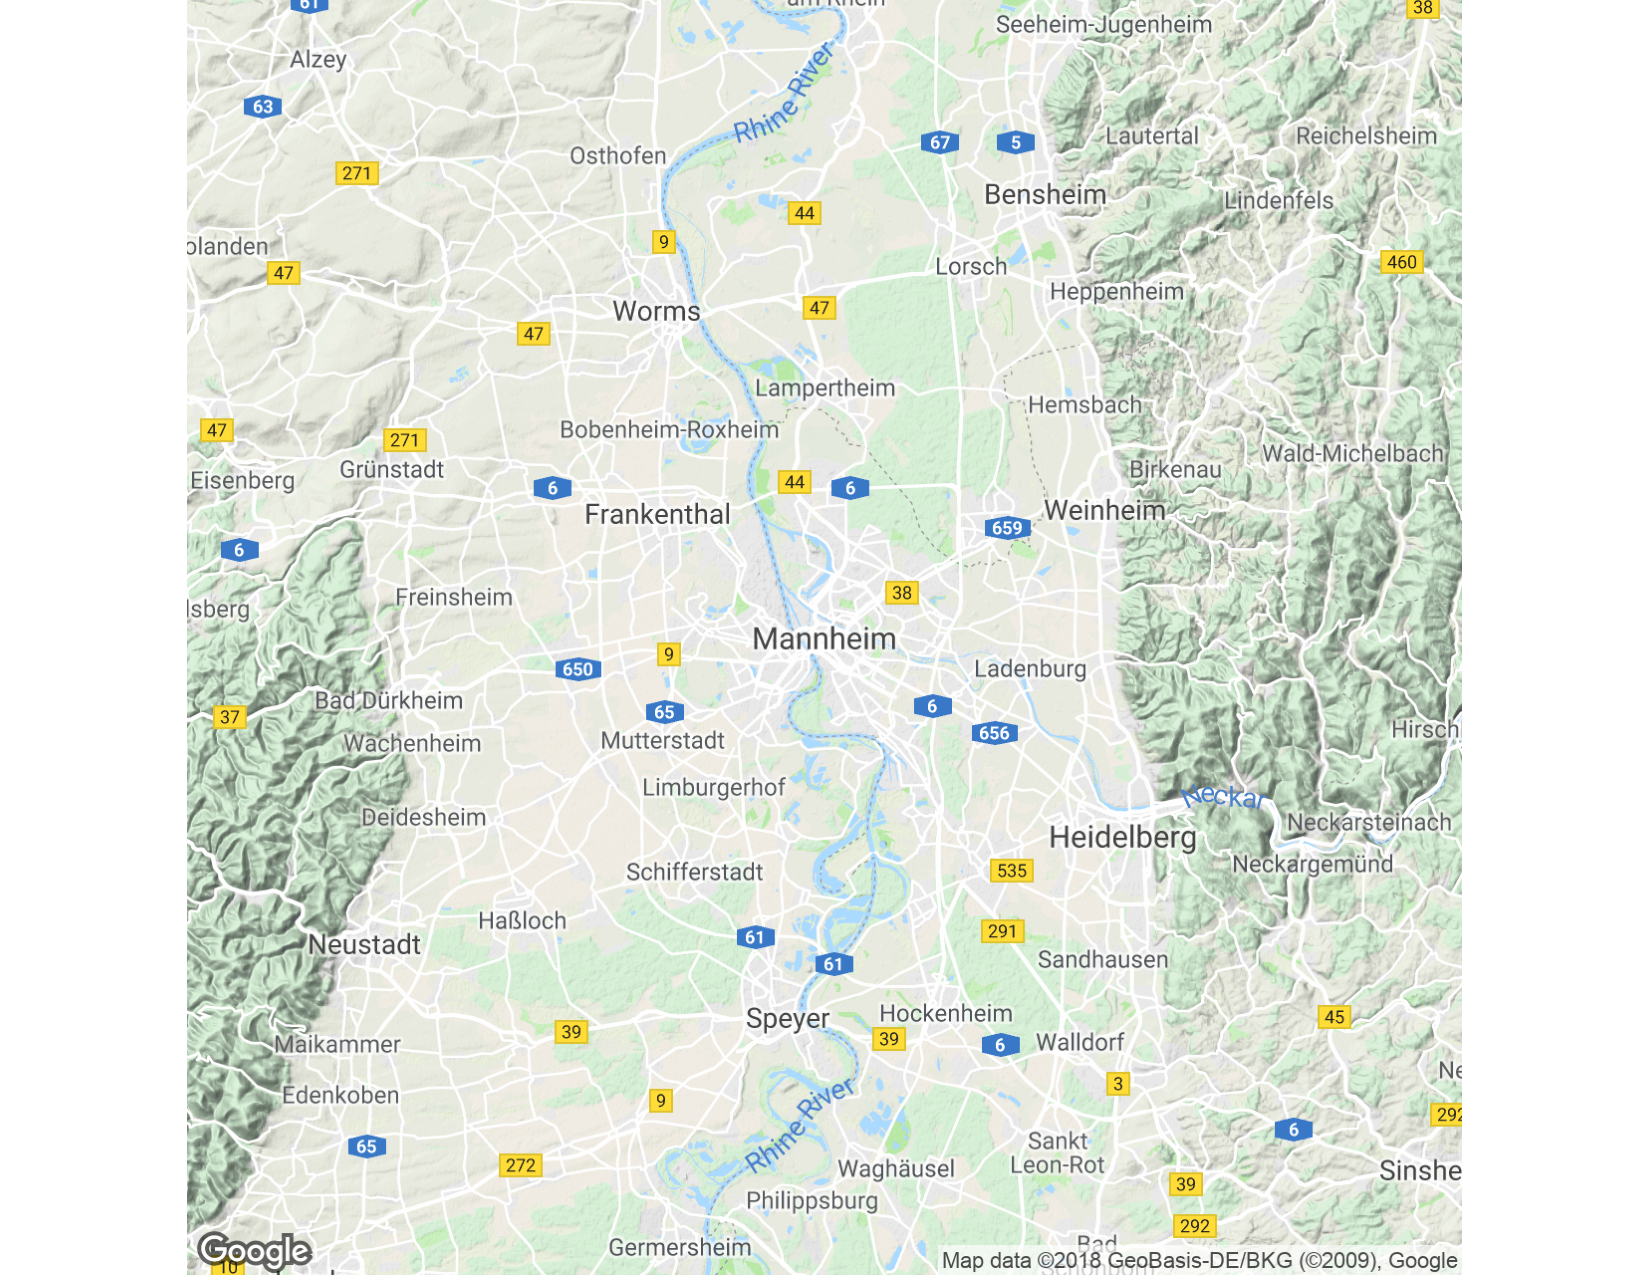
\includegraphics{figure/Mannheim_ggmap.pdf}

\end{frame}

\begin{frame}[fragile]{Karte für eine Sehenswürdigkeit}

\begin{Shaded}
\begin{Highlighting}[]
\KeywordTok{qmap}\NormalTok{(}\StringTok{"Berlin Brandenburger Tor"}\NormalTok{)}
\end{Highlighting}
\end{Shaded}

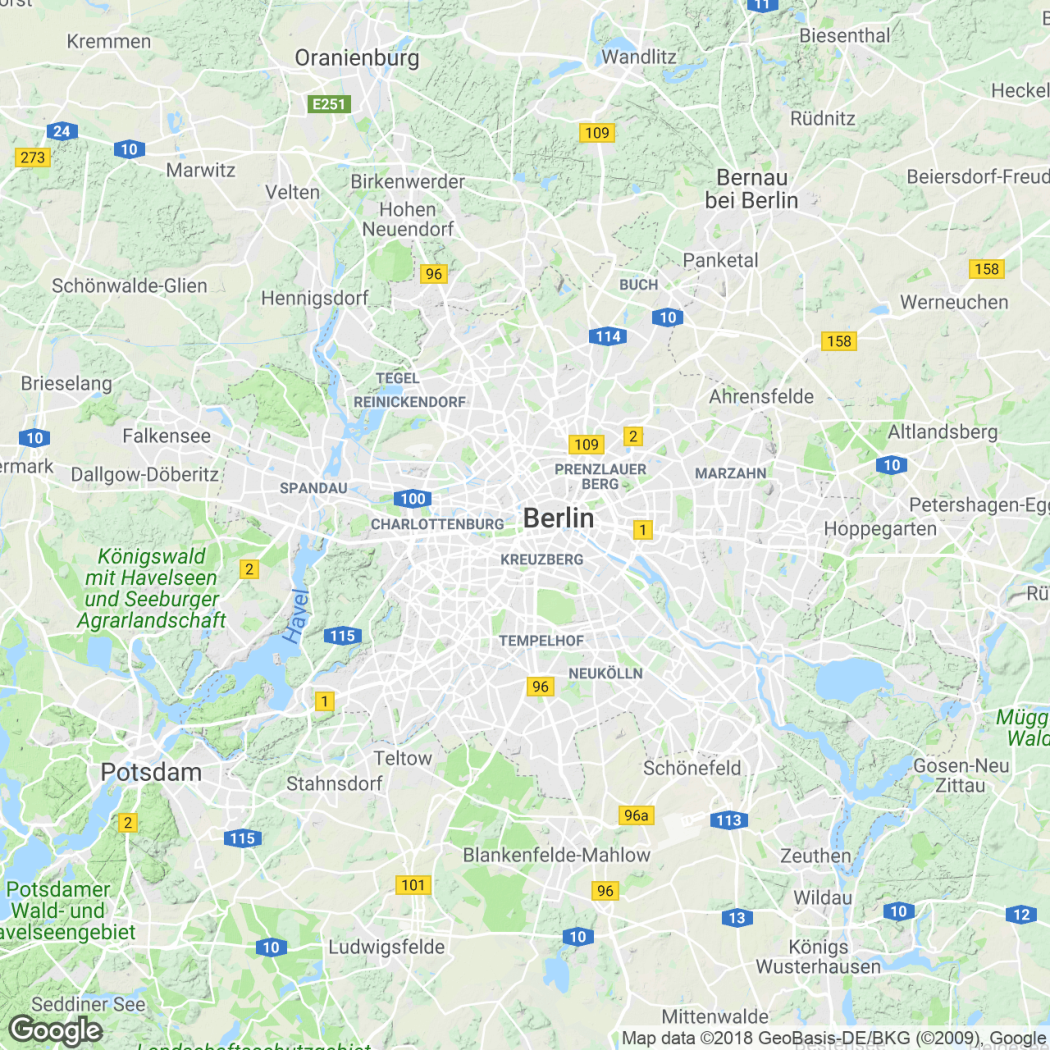
\includegraphics{figure/BBT_ggmap.pdf}

\end{frame}

\begin{frame}[fragile]{Karte für einen ganzen Staat}

\begin{Shaded}
\begin{Highlighting}[]
\KeywordTok{qmap}\NormalTok{(}\StringTok{"Germany"}\NormalTok{)}
\end{Highlighting}
\end{Shaded}

\begin{itemize}
\tightlist
\item
  Wir brauchen ein anderes \emph{zoom level}
\end{itemize}

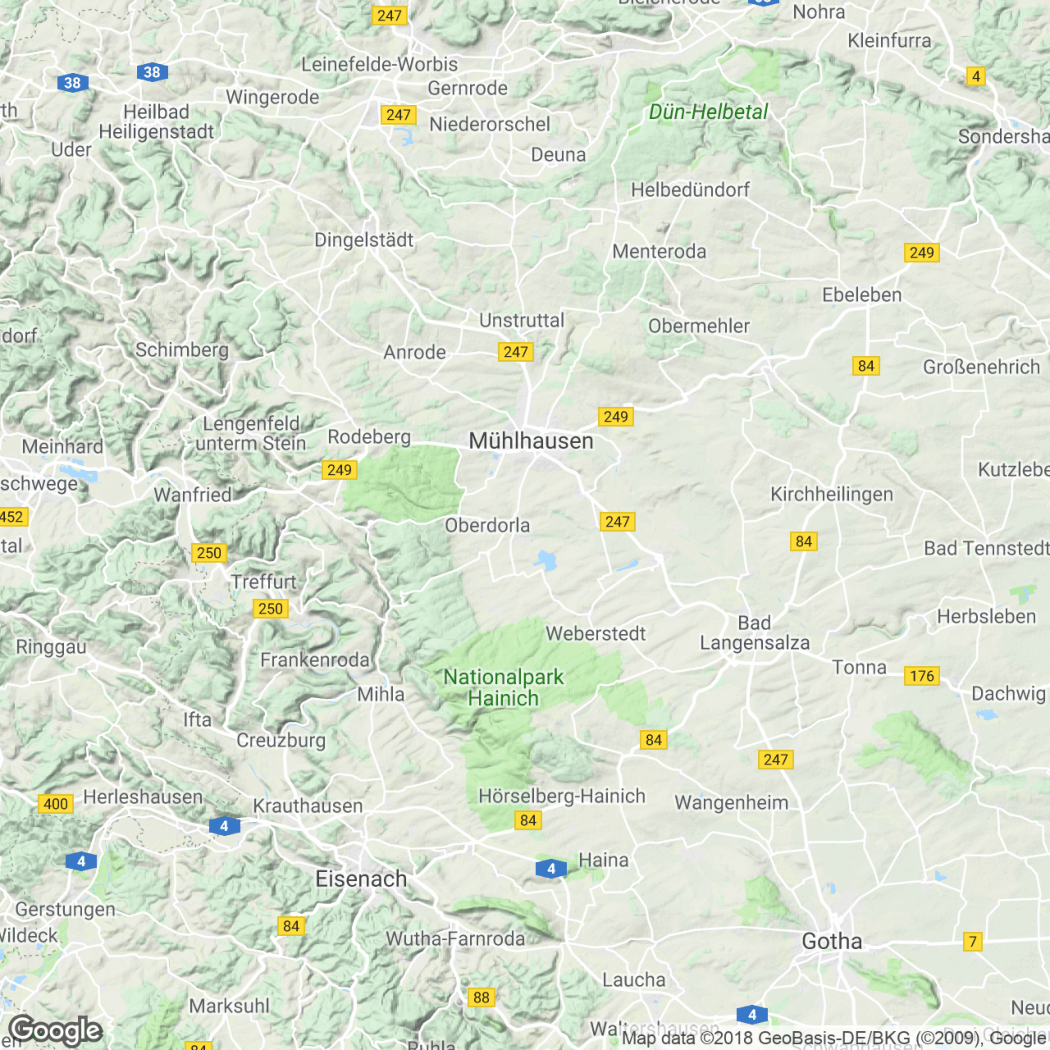
\includegraphics{figure/germany.pdf}

\end{frame}

\begin{frame}[fragile]{Ein anderes \emph{zoom level}}

\begin{itemize}
\tightlist
\item
  level 3 - Kontinent / level 10 - Stadt / level 21 - Gebäude
\end{itemize}

\begin{Shaded}
\begin{Highlighting}[]
\KeywordTok{qmap}\NormalTok{(}\StringTok{"Germany"}\NormalTok{, }\DataTypeTok{zoom =} \DecValTok{6}\NormalTok{)}
\end{Highlighting}
\end{Shaded}

\end{frame}

\begin{frame}[fragile]{Hilfe bekommen wir mit dem Fragezeichen}

\begin{Shaded}
\begin{Highlighting}[]
\NormalTok{?qmap}
\end{Highlighting}
\end{Shaded}

Verschiedene Abschnitte in der Hilfe:

\begin{itemize}
\tightlist
\item
  Description
\item
  Usage
\item
  Arguments
\item
  Value
\item
  Author(s)
\item
  See Also
\item
  Examples
\end{itemize}

\end{frame}

\begin{frame}[fragile]{Ganz nah dran}

\begin{Shaded}
\begin{Highlighting}[]
\KeywordTok{qmap}\NormalTok{(}\StringTok{'Mannheim'}\NormalTok{, }\DataTypeTok{zoom =} \DecValTok{20}\NormalTok{)}
\end{Highlighting}
\end{Shaded}

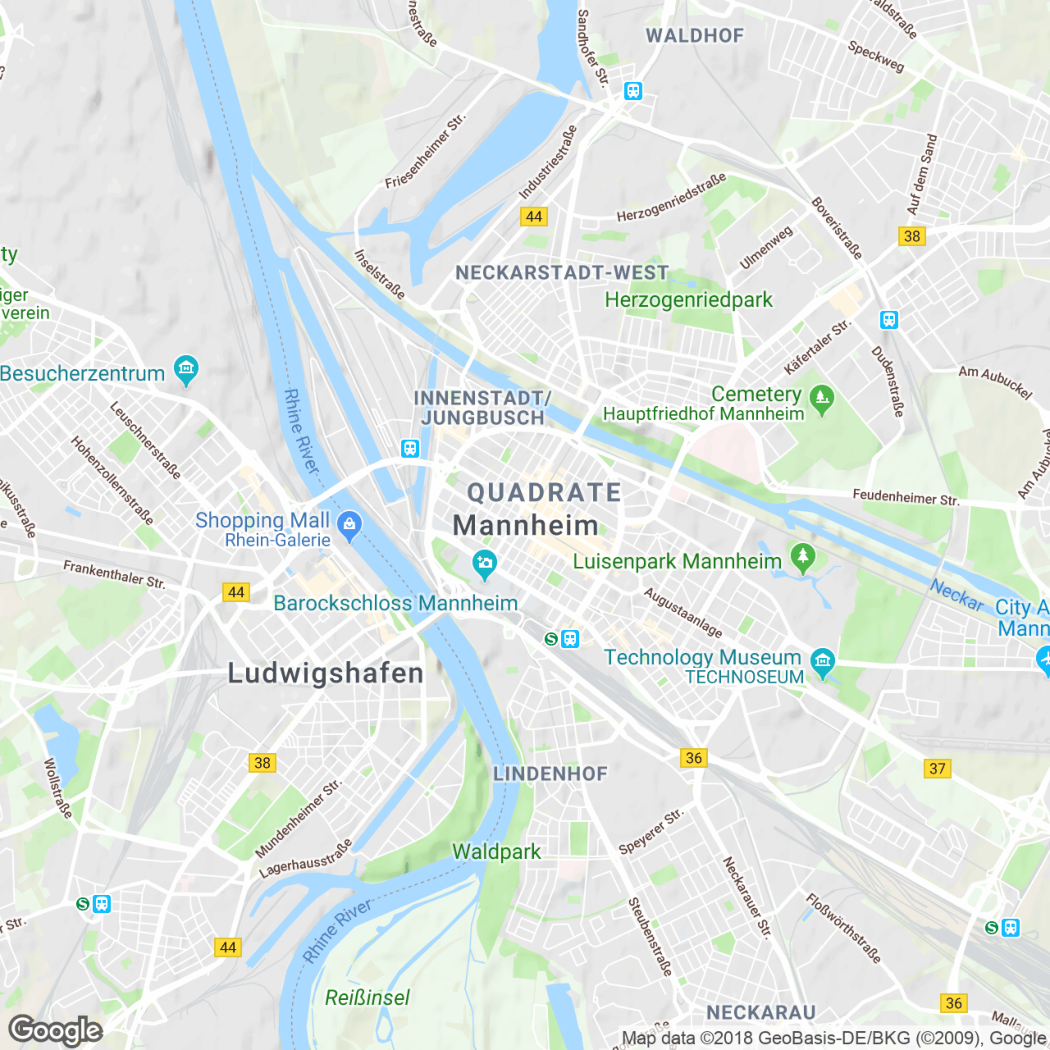
\includegraphics{figure/ham_map_z20.pdf}

\end{frame}

\begin{frame}[fragile]{\texttt{ggmap} - maptype satellite}

\begin{Shaded}
\begin{Highlighting}[]
\KeywordTok{qmap}\NormalTok{(}\StringTok{'Hamburg'}\NormalTok{, }\DataTypeTok{zoom =} \DecValTok{14}\NormalTok{, }\DataTypeTok{maptype=}\StringTok{"satellite"}\NormalTok{)}
\end{Highlighting}
\end{Shaded}

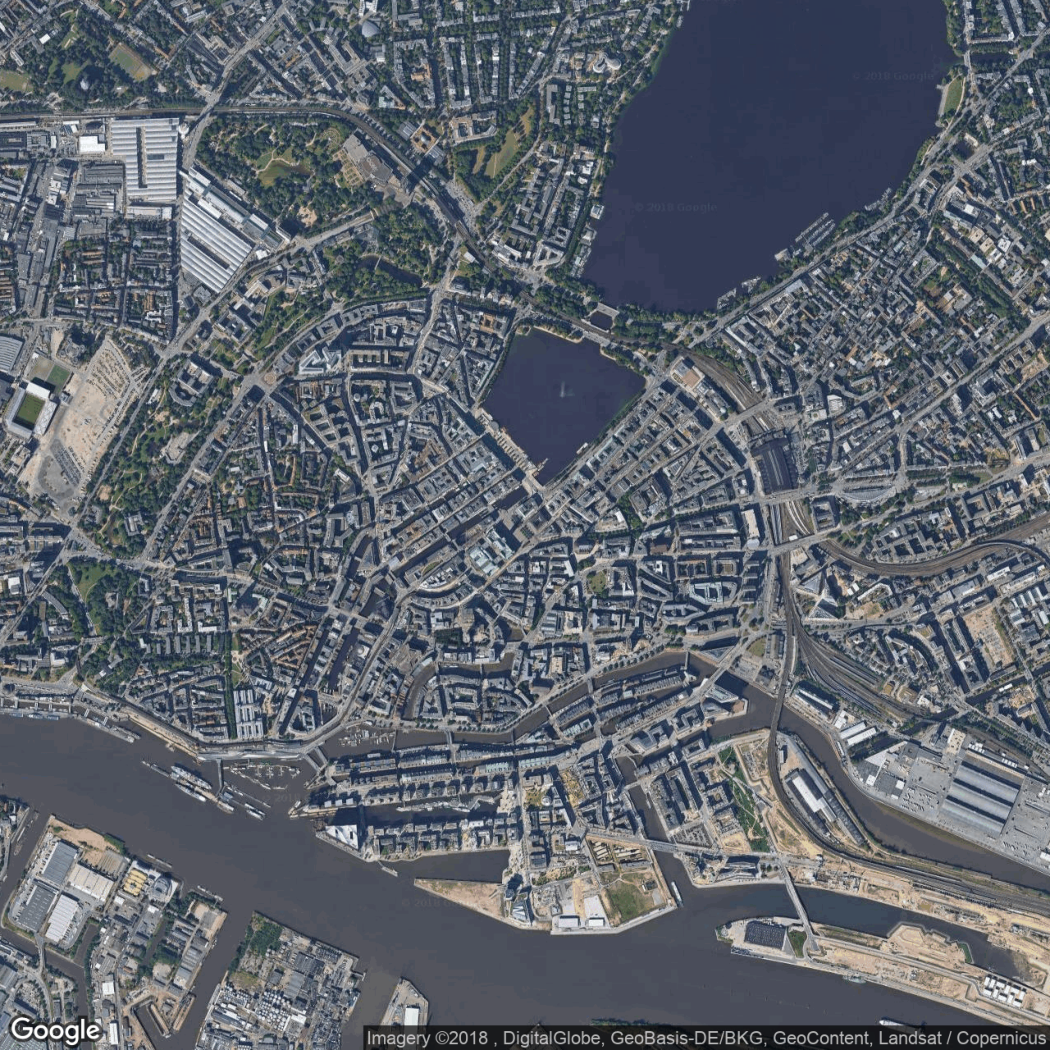
\includegraphics{figure/ham_map_sat.pdf}

\end{frame}

\begin{frame}[fragile]{\texttt{ggmap} - maptype satellite zoom 20}

\begin{Shaded}
\begin{Highlighting}[]
\KeywordTok{qmap}\NormalTok{(}\StringTok{'Hamburg'}\NormalTok{, }\DataTypeTok{zoom =} \DecValTok{20}\NormalTok{, }\DataTypeTok{maptype=}\StringTok{"hybrid"}\NormalTok{)}
\end{Highlighting}
\end{Shaded}

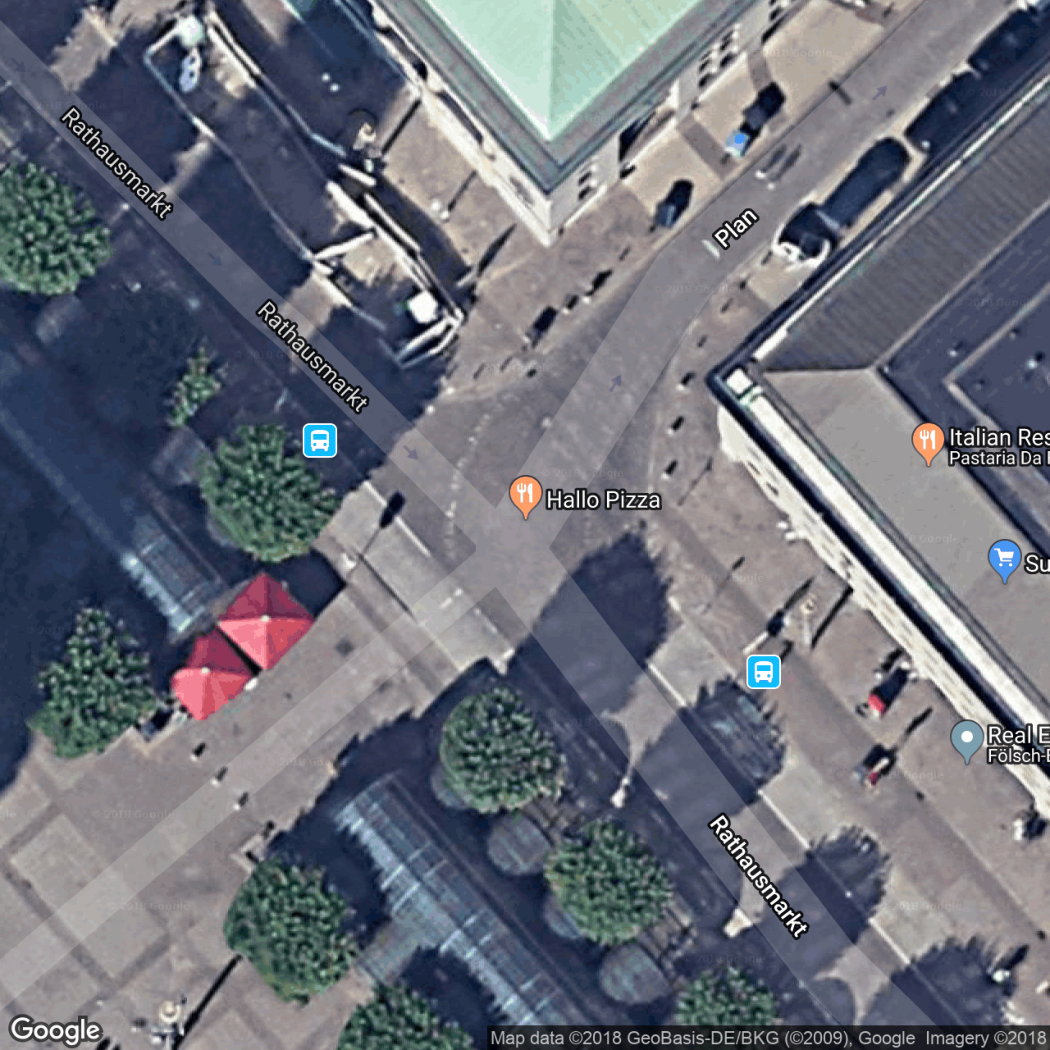
\includegraphics{figure/ham_map.pdf}

\end{frame}

\begin{frame}{Terrain/physical maps}

\begin{itemize}
\item
  Aus Physischen Karten kann man Informationen über Berge, Flüsse und
  Seen ablesen.
\item
  Farben werden oft genutzt um Höhenunterschiede zu visualisieren
\end{itemize}

\end{frame}

\begin{frame}{Abstrahierte Karten
(\href{http://www.designfaves.com/2014/03/abstracted-maps-reveal-cities-personalities}{http://www.designfaves.com})}

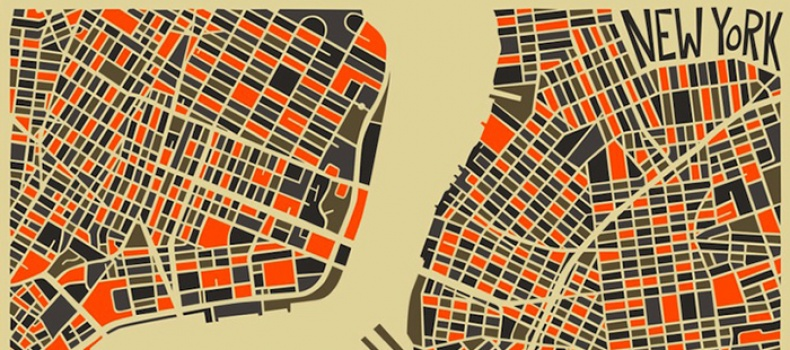
\includegraphics{figure/NYabstracted.jpg}

\begin{itemize}
\item
  Abstraktion wird genutzt um nur die essentiellen Informationen einer
  Karte zu zeigen.
\item
  Bsp. U-Bahn Karten - wichtig sind Richtungen und wenig Infos zur
  Orientierung
\item
  Im folgenden werden Karten vorgestellt, die sich gut als
  Hintergrundkarten eignen.
\end{itemize}

\end{frame}

\begin{frame}[fragile]{ggmap - maptype watercolor}

\begin{Shaded}
\begin{Highlighting}[]
\KeywordTok{qmap}\NormalTok{(}\StringTok{'Los Angeles'}\NormalTok{, }\DataTypeTok{zoom =} \DecValTok{14}\NormalTok{,}
 \DataTypeTok{maptype=}\StringTok{"watercolor"}\NormalTok{,}\DataTypeTok{source=}\StringTok{"stamen"}\NormalTok{)}
\end{Highlighting}
\end{Shaded}


\includegraphics{figure/lastamen.png}

\end{frame}

\begin{frame}{Graphiken speichern}

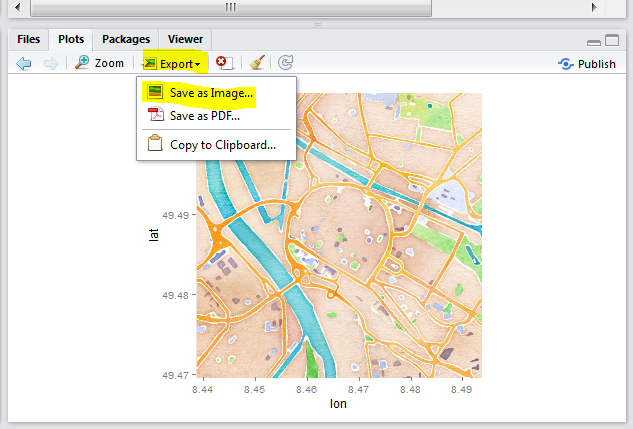
\includegraphics{figure/RstudioExport.PNG}

\end{frame}

\begin{frame}[fragile]{ggmap - ein Objekt erzeugen}

\begin{itemize}
\tightlist
\item
  \texttt{\textless{}-} ist der Zuweisungspfeil um ein Objekt zu
  erzeugen
\item
  Dieses Vorgehen macht bspw. Sinn, wenn mehrere Karten nebeneinander
  gebraucht werden.
\end{itemize}

\begin{Shaded}
\begin{Highlighting}[]
\NormalTok{MA_map <-}\StringTok{ }\KeywordTok{qmap}\NormalTok{(}\StringTok{'Mannheim'}\NormalTok{, }
               \DataTypeTok{zoom =} \DecValTok{14}\NormalTok{,}
               \DataTypeTok{maptype=}\StringTok{"toner"}\NormalTok{,}
               \DataTypeTok{source=}\StringTok{"stamen"}\NormalTok{)}
\end{Highlighting}
\end{Shaded}

\end{frame}

\begin{frame}[fragile]{\href{https://blog.dominodatalab.com/geographic-visualization-with-rs-ggmaps/}{Eine
Karte für die USA}}

\begin{Shaded}
\begin{Highlighting}[]
\NormalTok{usa_center =}\StringTok{ }\KeywordTok{as.numeric}\NormalTok{(}\KeywordTok{geocode}\NormalTok{(}\StringTok{"United States"}\NormalTok{))}
\NormalTok{USAMap =}\StringTok{ }\KeywordTok{ggmap}\NormalTok{(}\KeywordTok{get_googlemap}\NormalTok{(}\DataTypeTok{center=}\NormalTok{usa_center, }\DataTypeTok{scale=}\DecValTok{2}\NormalTok{, }\DataTypeTok{zoom=}\DecValTok{4}\NormalTok{), }\DataTypeTok{extent=}\StringTok{"normal"}\NormalTok{)}
\NormalTok{USAMap}
\end{Highlighting}
\end{Shaded}

\begin{Shaded}
\begin{Highlighting}[]
\KeywordTok{OSM_scale_lookup}\NormalTok{(}\DataTypeTok{zoom =} \DecValTok{10}\NormalTok{)}
\KeywordTok{qmap}\NormalTok{(}\DataTypeTok{location =} \StringTok{"Trier"}\NormalTok{, }\DataTypeTok{zoom =} \DecValTok{10}\NormalTok{, }\DataTypeTok{source =} \StringTok{"osm"}\NormalTok{,}\DataTypeTok{scale=}\DecValTok{575000}\NormalTok{)}
\end{Highlighting}
\end{Shaded}

\end{frame}

\begin{frame}{Cheatsheet}

\begin{itemize}
\tightlist
\item
  Cheatsheet zu
  \href{https://www.rstudio.com/wp-content/uploads/2015/04/ggplot2-cheatsheet.pdf}{data
  visualisation}
\end{itemize}

\url{https://www.rstudio.com/}

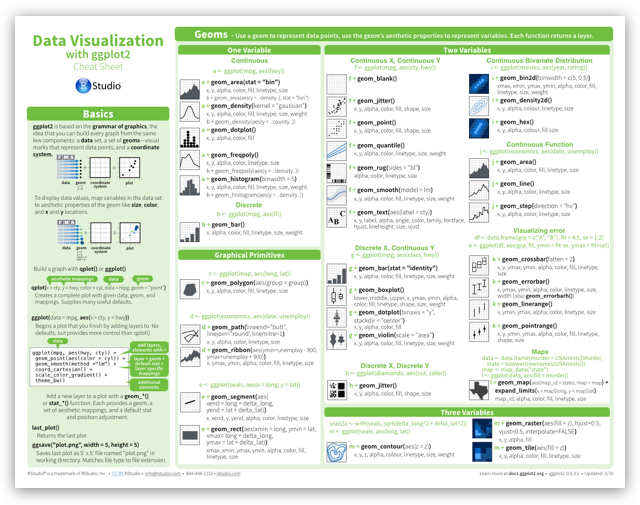
\includegraphics{figure/ggplot2-cheatsheet.png}

\end{frame}

\begin{frame}[fragile]{Resourcen und Literatur}

\begin{itemize}
\item
  Artikel von
  \href{http://journal.r-project.org/archive/2013-1/kahle-wickham.pdf}{\textbf{David
  Kahle und Hadley Wickham}} zur Nutzung von \texttt{ggmap}.
\item
  \href{http://rpackages.ianhowson.com/cran/ggmap/man/get_map.html}{\textbf{Schnell
  eine Karte bekommen}}
\item
  \href{http://www.kevjohnson.org/making-maps-in-r-part-2/}{\textbf{Karten
  machen mit R}}
\end{itemize}

\end{frame}

\end{document}
